%Version 3 December 2023
% See section 11 of the User Manual for version history
%
%%%%%%%%%%%%%%%%%%%%%%%%%%%%%%%%%%%%%%%%%%%%%%%%%%%%%%%%%%%%%%%%%%%%%%
%%                                                                 %%
%% Please do not use \input{...} to include other tex files.       %%
%% Submit your LaTeX manuscript as one .tex document.              %%
%%                                                                 %%
%% All additional figures and files should be attached             %%
%% separately and not embedded in the \TeX\ document itself.       %%
%%                                                                 %%
%%%%%%%%%%%%%%%%%%%%%%%%%%%%%%%%%%%%%%%%%%%%%%%%%%%%%%%%%%%%%%%%%%%%%

%%\documentclass[referee,sn-basic]{sn-jnl}% referee option is meant for double line spacing

%%=======================================================%%
%% to print line numbers in the margin use lineno option %%
%%=======================================================%%

%%\documentclass[lineno,sn-basic]{sn-jnl}% Basic Springer Nature Reference Style/Chemistry Reference Style

%%======================================================%%
%% to compile with pdflatex/xelatex use pdflatex option %%
%%======================================================%%

%%\documentclass[pdflatex,sn-basic]{sn-jnl}% Basic Springer Nature Reference Style/Chemistry Reference Style


%%Note: the following reference styles support Namedate and Numbered referencing. By default the style follows the most common style. To switch between the options you can add or remove “Numbered” in the optional parenthesis. 
%%The option is available for: sn-basic.bst, sn-vancouver.bst, sn-chicago.bst%  
 
%%\documentclass[pdflatex,sn-nature]{sn-jnl}% Style for submissions to Nature Portfolio journals
%%\documentclass[pdflatex,sn-basic]{sn-jnl}% Basic Springer Nature Reference Style/Chemistry Reference Style
\documentclass[pdflatex,sn-mathphys-num]{sn-jnl}% Math and PhysicalSciences Numbered Reference Style 
%%\documentclass[pdflatex,sn-mathphys-ay]{sn-jnl}% Math and Physical Sciences Author Year Reference Style
%%\documentclass[pdflatex,sn-aps]{sn-jnl}% American Physical Society (APS) Reference Style
%%\documentclass[pdflatex,sn-vancouver,Numbered]{sn-jnl}% Vancouver Reference Style
%%\documentclass[pdflatex,sn-apa]{sn-jnl}% APA Reference Style 
%%\documentclass[pdflatex,sn-chicago]{sn-jnl}% Chicago-based Humanities Reference Style

%%%% Standard Packages
%%<additional latex packages if required can be included here>



\usepackage[utf8]{inputenc}
\usepackage{tcolorbox}
\usepackage{titlesec}
\usepackage{geometry}
\usepackage{array}
\usepackage{algorithmic}
\usepackage{graphicx}%
\usepackage{multirow}%
\usepackage{amsmath,amssymb,amsfonts}%
\usepackage{enumitem}
\usepackage{amsthm}%
\usepackage{mathrsfs}%
\usepackage[title]{appendix}%
\usepackage{xcolor}%
\usepackage{textcomp}%
\usepackage{manyfoot}%
\usepackage{booktabs}%
\usepackage{algorithm}%
\usepackage{algorithmicx}%
\usepackage{algpseudocode}%
\usepackage{listings}%
%%%%

%%%%%=============================================================================%%%%
%%%%  Remarks: This template is provided to aid authors with the preparation
%%%%  of original research articles intended for submission to journals published 
%%%%  by Springer Nature. The guidance has been prepared in partnership with 
%%%%  production teams to conform to Springer Nature technical requirements. 
%%%%  Editorial and presentation requirements differ among journal portfolios and 
%%%%  research disciplines. You may find sections in this template are irrelevant 
%%%%  to your work and are empowered to omit any such section if allowed by the 
%%%%  journal you intend to submit to. The submission guidelines and policies 
%%%%  of the journal take precedence. A detailed User Manual is available in the 
%%%%  template package for technical guidance.
%%%%%=============================================================================%%%%

%% as per the requirement new theorem styles can be included as shown below
\theoremstyle{thmstyleone}%
\newtheorem{theorem}{Theorem}%  meant for continuous numbers
%%\newtheorem{theorem}{Theorem}[section]% meant for sectionwise numbers
%% optional argument [theorem] produces theorem numbering sequence instead of independent numbers for Proposition
\newtheorem{proposition}[theorem]{Proposition}% 
%%\newtheorem{proposition}{Proposition}% to get separate numbers for theorem and proposition etc.

\theoremstyle{thmstyletwo}%
\newtheorem{example}{Example}%
\newtheorem{remark}{Remark}%

\theoremstyle{thmstylethree}%
\newtheorem{definition}{Definition}%

\raggedbottom
%%\unnumbered% uncomment this for unnumbered level heads





% Define a special formatting only for titleonlybox
\newtcolorbox{titleonlybox}{%
    colback=blue!50!white, % Lighter blue background
    colframe=blue!50!white, % Lighter blue border
    fontupper=\bfseries\scriptsize\color{black}, % Black text for better contrast
    sharp corners,
    width=\columnwidth, % Full column width
    height=4mm, % Adjusted height for better fit
    boxrule=0pt, % No extra border
    before=\vspace{2pt}, % Minimal vertical space
    after=\vspace{2pt},  % Minimal vertical space
    halign=left, % Horizontally center the text
    valign=center, % Vertically center the text
    before upper={%
        % Apply special title format only inside this box
        \titleformat{\section}
          {\large\bfseries}{\thesection.}{0.5em}{}
        \titleformat{\subsection}
          {\normalsize\bfseries}{\thesubsection.}{0.5em}{}
        \titleformat{\subsubsection}
          {\normalsize}{\thesubsubsection.}{0.5em}{}
    }
}

% Define a custom section format for custombox
\newtcolorbox[auto counter, number within=section]{custombox}[2][]{%
    colback=blue!10, % Even lighter blue background
    colframe=blue!40!white, % Lighter blue frame
    fonttitle=\bfseries\scriptsize, % Smaller title font
    title=#2,
    left=2mm,
    right=2mm,
    top=1mm,
    bottom=1mm,
    sharp corners,
    width=\columnwidth,
    enhanced,
    before=\vspace{2pt}, % Reduced vertical space before the box
    after=\vspace{2pt},  % Reduced vertical space after the box
    before upper={%
        % Apply special title format only inside this box
        \titleformat{\section}
          {\large\bfseries}{\thesection.}{0.5em}{}
        \titleformat{\subsection}
          {\normalsize\bfseries}{\thesubsection.}{0.5em}{}
        \titleformat{\subsubsection}
          {\normalsize}{\thesubsubsection.}{0.5em}{}
    }
}










\begin{document}

\title[Article Title]{Design of a Unified Quantum-Resistant and AI-Enabled Healthcare Network with Blockchain Security}

%%=============================================================%%
%% GivenName	-> \fnm{Joergen W.}
%% Particle	-> \spfx{van der} -> surname prefix
%% FamilyName	-> \sur{Ploeg}
%% Suffix	-> \sfx{IV}
%% \author*[1,2]{\fnm{Joergen W.} \spfx{van der} \sur{Ploeg} 
%%  \sfx{IV}}\email{iauthor@gmail.com}
%%=============================================================%%

\author[1]{\fnm{Utsa} \sur{Das}}\email{dasutsa102@gmail.com}

\author[2]{\fnm{Sourav} \sur{Banerjee}}\email{mr.sourav.banerjee@ieee.org}

\author[3]{\fnm{Debashis} \sur{Das}}\email{debashis.das@ieee.org}

\author[4]{\fnm{Manju} \sur{Biswas}}\email{csemanju@gmail.com
}

\author[5]{\fnm{Kousik} \sur{Dasgupta}}\email{kousik.dasgupta@kgec.edu.in}





\affil[1,2,4,5]{\orgdiv{Computer Science and Engineering}, \orgname{Kalyani Government Engineering College}, \orgaddress{\city{Kalyani}, \postcode{741235}, \state{WB}, \country{India}}}

\affil[3]{\orgdiv{Computer Science and Data Science}, \orgname{Meharry Medical College}, \orgaddress{\city{Nashville}, \postcode{37208}, \state{TN}, \country{USA}}}


%%==================================%%
%% Sample for unstructured abstract %%
%%==================================%%







%%%%%% Utso Start you from here  %%%%%%%%%%%%%%

\abstract{The healthcare industry is undergoing a digital transformation, with increasing reliance on interconnected devices, electronic health records (EHRs), and remote monitoring systems. However, this evolution brings critical challenges such as data breaches, lack of interoperability, insecure communication, delayed diagnostics, and the looming threat of quantum-enabled cyberattacks. Traditional security frameworks and centralized systems are proving insufficient in protecting sensitive patient data and ensuring real-time protection. This paper proposes a next-generation architecture for smart healthcare networks that integrates Artificial Intelligence (AI), Blockchain, and Quantum Computing to overcome these pressing limitations. AI is employed for intelligent diagnostics, real-time monitoring, and predictive analytics. Blockchain ensures immutable, decentralized, and auditable data sharing across stakeholders. Quantum-safe cryptography and the exploration of quantum computing enhance the system’s resistance against emerging cryptographic threats and optimize complex decision-making processes. Together, these components establish a robust, scalable, and quantum-resilient platform for next-generation healthcare delivery. The proposed framework gives a comprehensive solution to the current challenges in digital healthcare by ensuring intelligent decision-making, secure data management, and future-proof protection against evolving cyber threats. It empowers healthcare providers with AI-driven insights for early diagnosis and efficient care delivery, while blockchain guarantees the integrity, transparency, and privacy of sensitive medical data through decentralized mechanisms.}

\keywords{Quantum Machine Learning(QML), Quantum Neural Networks(QNN), Artificial Intelligence(AI), Quantum Key Distribution (QKD), Post-Quantum Cryptography, Blockchain, Electronic Healthcare Records(EHRs)}


\maketitle

\section{Introduction}
The rise of digital healthcare besides advancements of EHRs\cite{bib4} and telemedicine causes sensitive patient medical data susceptible to cyber attacks.Traditional security measures being no longer reliable,there is need for advanced solutions. Quantum technologies specially quantum cryptography provide robust encryption. It uses principles of quantum mechanics to achieve hypothetically unbreakable security. QKD protocols\cite{bib5} like BB84 and E91 ensure secure communications and can detect eavesdropping attempts in real-time.Besides quantum technology,AI can improve security through machine learning models that will predict errors, detect anomalies and minimizing threats in real-time.Security systems supervised by AI models can dynamically adapt to new attack patterns. Moreover, Blockchain can provide an immutable and transparent ledger that will ensure that data integrity and access control. are properly managed. This prevent unauthorized alterations to electronic healthcare records.These technologies have high potential but their integration into healthcare systems has several challenges. High implementation costs, compatibility with existing infrastructures, operations and management are still areas that provide challenges.To address these issues,we require advanced frameworks that will integrate quantum, AI, and Blockchain. This paper proposes a novel approach to combine Quantum Key Distribution (QKD), federated learning (AI), and \textbf{blockchain} for more secure and distributed healthcare systems.


\subsection{Contributions of This Paper}
This paper makes the following key contributions:
To ensure the security of healthcare in the future, this paper provides an example of framework to integrate AI, Blockchain and Quantum. Firstly it provides an AI based  authentication system(quantum secure) that uses quantum key distribution(QKD) for secured communication and also post quantum cryptography to ensure the protection of data against threats of quantum computing. Secondly the paper provides a mechanism of decentralized access for patient records using Blockchain to ensure the integrity, transparency and auditability of data. Thirdly it integrates AI driven anomaly detection models that will identify irregular access pattern in real time and will improve the system's ability in prevention of unauthorised access. Moreover it proposes a hybrid framework for encryption that combines both classical and quantum safe algorithms to protect sensitive health data making it future proof. The proposed system offers a comprehensive solution to healthcare security by addressing both the present as well as the future cybersecurity challenges. It provides a resilient, scalable model that is quantum resistant for making exchange of healthcare information secure.
The goal of this paper is to address these aspects in order to contribute to the advancement of secure resilient scalable and future proof healthcare systems.


\section{Background and Related Work}

The stringent requirements for safeguarding Electronic Health Records (EHRs) in the face of modern cybersecurity threats necessitate a departure from traditional methods. Security protocols that based solely on classical cryptography and centralized access control mechanisms are vulnerable to attacks from quantum computing and sophisticated AI models. Okwudili Matthew Ugochukwu et al. \cite{bib4} highlights the critical intersection of cybersecurity, sensitive data handling, and regulatory compliance within electronic healthcare systems. 
Blockchain technology has emerged as a promising solution for ensuring data integrity and transparency. Kasyapa et al. (2024) \cite{bib8} provided a comprehensive investigation into blockchain use cases in healthcare. It highlightedits potential to mitigate performance issues through decentralized architectures. Sengupta et al. (2024) \cite{bib7} analyzed the energy efficiency of blockchain networks. However, these studies did not address the integration of quantum-resistant cryptographic techniques or AI-driven security intelligence.

Nankya et al. (2024) \cite{bib10} reviewed AI and machine learning techniques for enhancing security in E-health systems. It discussed their effectiveness in detection of unauthorized access patterns. But centralized AI models still remain susceptible to adversarial manipulation and data privacy risks, necessitating decentralized approaches which implement blockchain for secure data sharing.

Quantum Key Distribution (QKD) highly advances cryptographic security by using quantum mechanics to provide hypothetically unbreakable encryption. Radanliev (2024) \cite{bib11} explored the application of QKD protocols like BB84 and E91 in clinical data exchange. It presented their ability to detect eavesdropping attempts through quantum state disturbance analysis. Sharma et al. (2024) \cite{bib16} proposed QIoTChain, a fusion of quantum IoT and blockchain for advanced data protection in Industry 4.0. But its deployment in healthcare systems remains underexplored.

Several researches have attempted to address cybersecurity challenges in healthcare. Bathula et al. (2024) \cite{bib6} introduced the concept of integrating blockchain, AI and healthcare systems but did not incorporate quantum cryptography into their framework. Shahsavari et al. (2024) \cite{bib9} explored the integration of federated learning with blockchain for privacy-preserving healthcare applications. Yet it faced scalability challenges due to high computational overheads.

 Unlike previous studies that focus on individual technologies or partial integrations this paper addresses the critical gaps by combining post-quantum cryptography with decentralized architectures and intelligent monitoring systems. Through usage of NTRU-enhanced biometric authentication, Merkle tree-based data integrity verification and QKD-optimized key exchange protocols this framework ensures more advanced protection against both classical and quantum threats while maintaining operational efficiency and regulatory compliance.


\section{Proposed Frameworks}
Artificial Intelligence (AI) and Blockchain are transforming healthcare security \cite{bib6} by enhancing threat detection. This allow secure data exchange and its main advantage is that it enables  decentralized access control . AI models process large datasets \(D = \{x_1, x_2, \ldots, x_n\}\) to identify anomalies and detect threats in real-time. Anomaly detection involves calculating deviations from normal behavior using the equation:


\begin{equation}
\text{Anomaly Score} = \frac{\sum_{i=1}^n |x_i - \mu|}{n}, 
\end{equation}


where \(\mu\) is the mean of the dataset. Threats are flagged if the anomaly score exceeds a predefined threshold.

AI-driven intrusion detection uses classification models. The probability of an attack is given as:
\begin{equation}
P(\text{Threat} | x) = \frac{1}{1 + e^{-z}}, 
\end{equation}
with \(z = \beta_0 + \sum_{i=1}^m \beta_i x_i\). However, AI models are susceptible to adversarial attacks. Attackers modify input \(x\) with adversarial noise \(\epsilon\) to mislead the system:
\begin{equation}
x' = x + \epsilon.
\end{equation}

Federated Learning (FL) mitigates these risks by training AI models across multiple devices besides preserving data privacy\cite{bib9}. The global model is updated using the formula:
\begin{equation}
w_t = \sum_{k=1}^K \frac{n_k}{N} w_t^k, 
\end{equation}
where \(w_t\) is the global model, \(w_t^k\) is the local model, and \(N\) is the total dataset size.

To ensure integrity AI models can be integrated with Blockchain \cite{bib6}. Blockchain operates on a distributed ledger where transactions are cryptographically hashed\cite{bib7}:
\begin{equation}
H_i = \text{SHA-256}(T_i), 
\end{equation}
where \(H_i\) represents the transaction hash. The Merkle root efficiently summarizes transactions\cite{bib7}:
\begin{equation}
\text{Root Hash} = H(H_1 || H_2 || \ldots || H_n).
\end{equation}

Smart contracts automate security protocols based on predefined conditions as follows:
\begin{equation}
f(x) = 
\begin{cases} 
1, & C(x) = \text{True}, \\
0, & \text{otherwise}.
\end{cases}
\end{equation}

Blockchain ensures patient record exchange is securely done:
\begin{equation}
I = H(D) \oplus \text{Signature},
\end{equation}
where \(D\) is data and \(\oplus\) represents verification.

Patient-controlled data access is protected using encryption strategy:
\begin{equation}
E_k(D) = D', \quad D = D' \cdot k^{-1}.
\end{equation}

Federated systems integrate Blockchain \cite{bib9}for secure collaboration across multiple parties using decentralized mechanism:
\begin{equation}
P_i = \frac{S_i}{\sum_{j=1}^n S_j},
\end{equation}
where \(P_i\) is the selection probability of participant \(i\), and \(S_i\) is their stake.

Blockchain improves scalability in healthcare security. The network throughput is given by\cite{bib8}:

\begin{equation}
  T = \frac{\text{Number of Transactions per Block} \cdot \text{Block Rate}}{\text{Block Size}}  
\end{equation}

\noindent Where:
 T = Throughput (Transactions per second), Number of Transactions per Block = The number of transactions included in each block, Block Size = The block size in MB.

\noindent Block Rate = The rate at which new blocks are added to the blockchain (blocks per second)

The integration of AI, Federated Learning, and Blockchain enhances cybersecurity in healthcare. It provides decentralized mechanism to control access, make data exchange secure and allow real-time threat detection. This ensures compliance with privacy regulations such as GDPR and HIPAA\cite{bib10}.

Quantum mechanics advances healthcare security by integrating with blockchain and AI-based mechanisms\cite{bib11,bib12}, ensuring protection against both classical and quantum threats. When applied to healthcare, quantum encryption ensures that sensitive patient data remains protected from both current and future computational vulnerabilities arising due to the advent of quantum computing.  

Quantum Key Distribution (QKD) protocols such as BB84 and E91 is used for secure encryption key transmission. This uses properties like quantum entanglement and superposition, enabling secure key exchange between healthcare providers and patients while detecting eavesdropping attempts. The no-cloning theorem ensures key integrity. The Heisenberg uncertainty principle prevents undetected interception depicted as follows 

\begin{equation}  
\Delta x \cdot \Delta p \geq \frac{\hbar}{2},  
\end{equation}  

where \( \Delta x \) and \( \Delta p \) indicate uncertainties in position and momentum and \( \hbar \) indicates the reduced Planck's constant. Any attempt at measurement introduces uncertainty, helping detect an eavesdropper.  

Post-quantum cryptography techniques strengthen encryption security. Lattice-based encryption such as NTRU provides strong resistance against quantum attacks\cite{bib12}. It operates through polynomial rings where encryption is defined as: 

\begin{equation}  
\mathbf{a} = \mathbf{e} \cdot \mathbf{f} + \mathbf{g} \pmod{q},  
\end{equation}  

where \( \mathbf{a} \) represents encrypted data, \( \mathbf{e} \) is the error vector, \( \mathbf{f} \) is the private key, and \( \mathbf{g} \) is the public key. This system ensures that an adversary cannot feasibly decrypt patient health data despite quantum computational capabilities.  

Secure hybrid quantum-classical communication channels further enhance security by using entangled photons to detect eavesdropping. This is verified through Bell’s inequality,  

\begin{equation}  
S = |E(a, b) - E(a, b') + E(a', b) + E(a', b')| \leq 2,  
\end{equation}  

where \( E(a, b) \) represents correlation measurements across different settings. Violation of this inequality confirms entanglement. This is crucial for secure key exchange. Quantum signatures also allow authentication of both patients and healthcare providers. Thus it replaces traditional authentication methods such as passwords or biometrics, which are susceptible to interception or spoofing.  

Quantum-secured blockchain mechanisms further enhance data integrity by employing post-quantum encrypted decentralized storage. Blockchain transactions in healthcare are validated using quantum-resistant consensus mechanisms. This includes the Quantum Byzantine Agreement (QBA), ensuring security even against quantum adversaries.  

Quantum Machine Learning (QML)\cite{bib13} models trained on quantum computers improve anomaly detection. It also identifies unusual access patterns and potential data breaches more effectively than classical methods. One such example is Grover’s algorithm that provides a quadratic speedup for unstructured search. It reduces the complexity to  

\begin{equation}  
T = O(\sqrt{N}),  
\end{equation}  

where \( T \) is the number of iterations required to locate an anomaly in a dataset of size \( N \). This highly improves real-time breach detection and response in healthcare security.  

By integrating these quantum technologies, healthcare security gains and multi-layer defense mechanism, it ensures resilience against emerging computational threats.  


\begin{figure}[t]
\centering
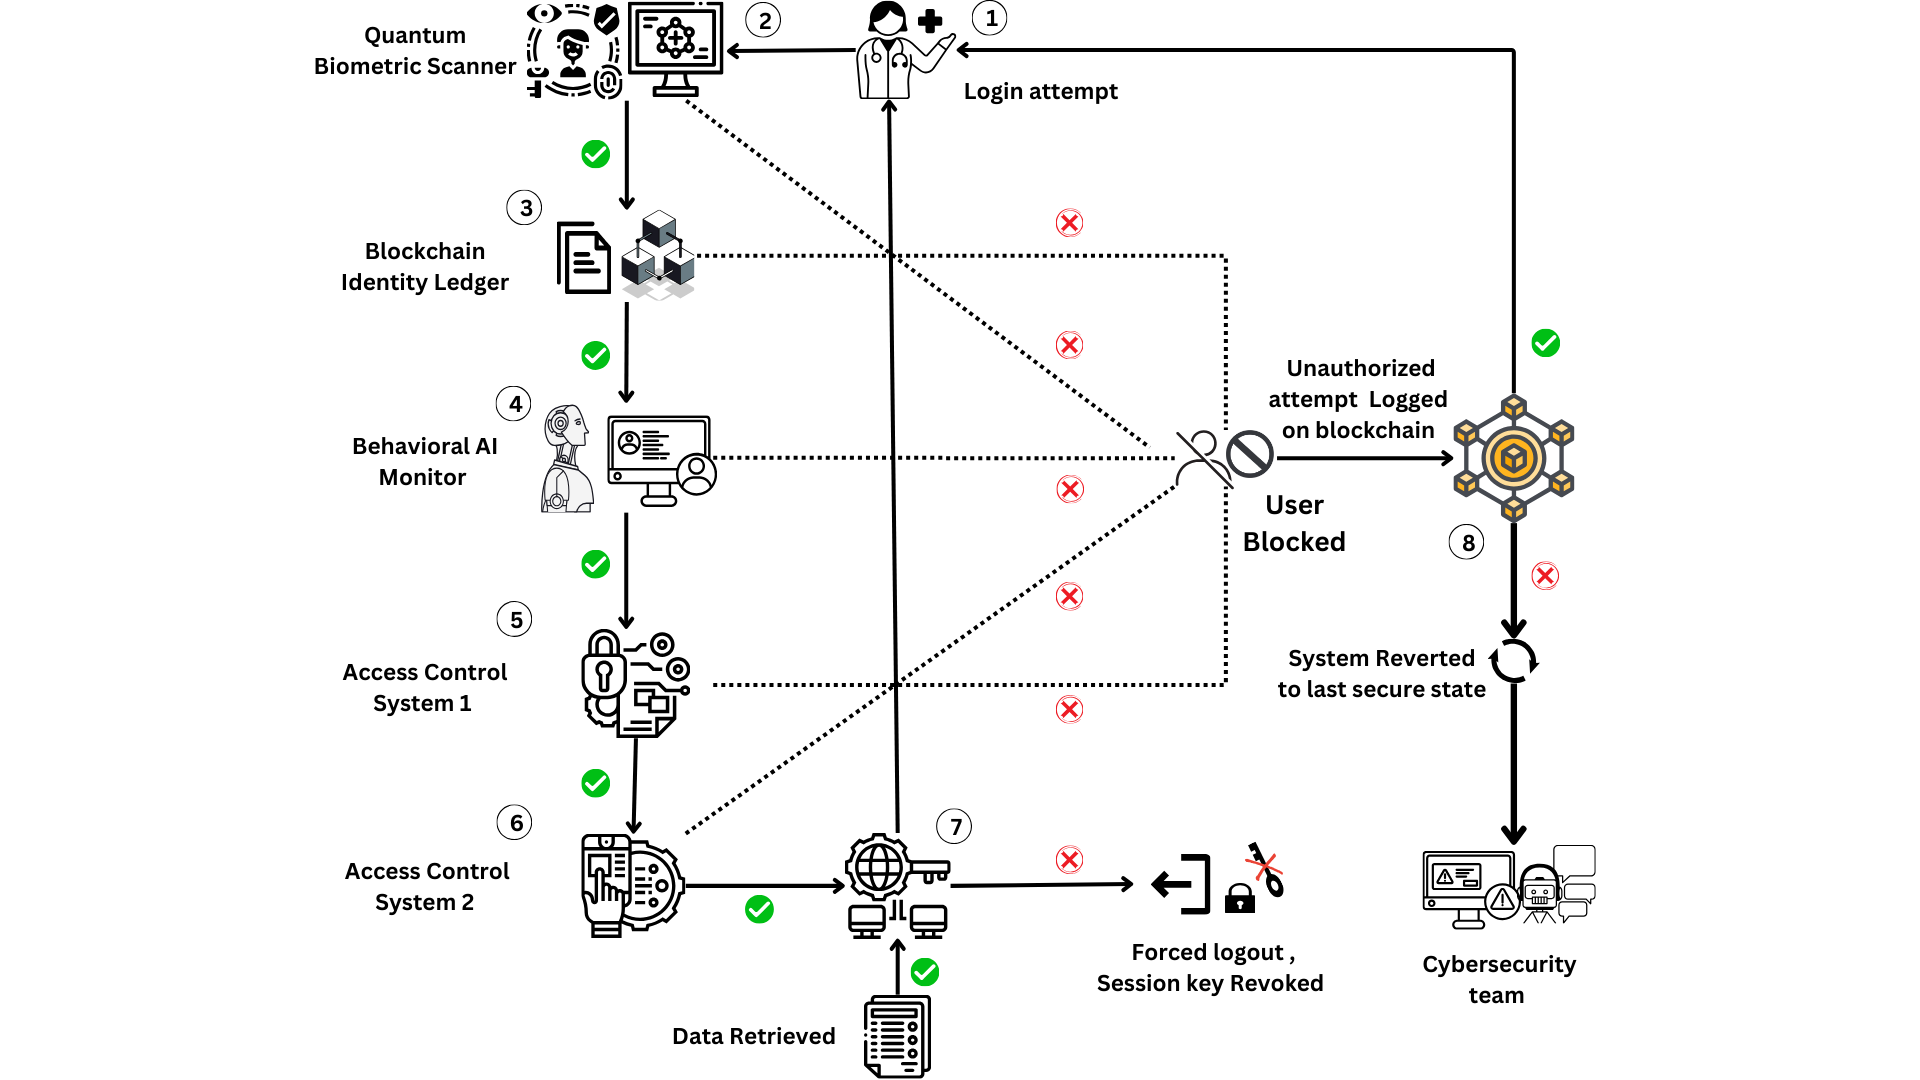
\includegraphics[width=13cm]{User Authenticationing.png}
\centering
\caption{Ultra-Secure User Authentication and Access Control.}
  \label{fig:User_Authentication}
\end{figure}


%%%%%%%%%%%%%%%%%%%%%%%%%%%%%%%%%%%%%%%%%%%%%%%%%%%%%

\section{Methodology}

%%%%%%%%%%%%%%%%%%%%%%%%%%%%%%%%%%%%%%%%%%%%%%%%%%%%%



\subsection{User Authentication}
To implement secure user authentication the system utilizes a blockchain based ledger as shown in Fig. \ref{fig:User_Authentication}. It stores hashed credentials of user (\texttt{user\_id}, \texttt{user\_token}) and biometric data\cite{bib14}. A decentralized authentication protocol ensures validation of tokens through smart contracts. Once user logs in, the blockchain network retrieves and verifies the \texttt{user\_token} and \texttt{user\_id} against the ledger. An biometric authentication module, supported by AI is simultaneously used. A convolutional neural network (CNN) that is pre-trained on diverse biometric dataset, analuzes the user’s input (\texttt{biometric\_data}) and ensures a match with the encrypted reference tht is stored on the blockchain.On failure of a verification the system returns ``Access Denied". For session integrity, quantum key distribution (QKD) is implemented to exchange symmetric keys between the system and the user\cite{}. BB84 or E91 protocol is simulated through usage of quantum communication libraries\cite{bib16}. This verifies key integrity against attempts to tamper. Proper aunthentication at each layer including credentials, biometrics and QKD will stimulate a blockchain transaction. It will cause logging the event for detection of pecularity and regulatory compliance.


%%%%%%%%%%%%%%%%%%%%%%%%%%%%%%%%%%%%%%%%%%%%%%%%%%%%%

\begin{figure}[t]
\centering
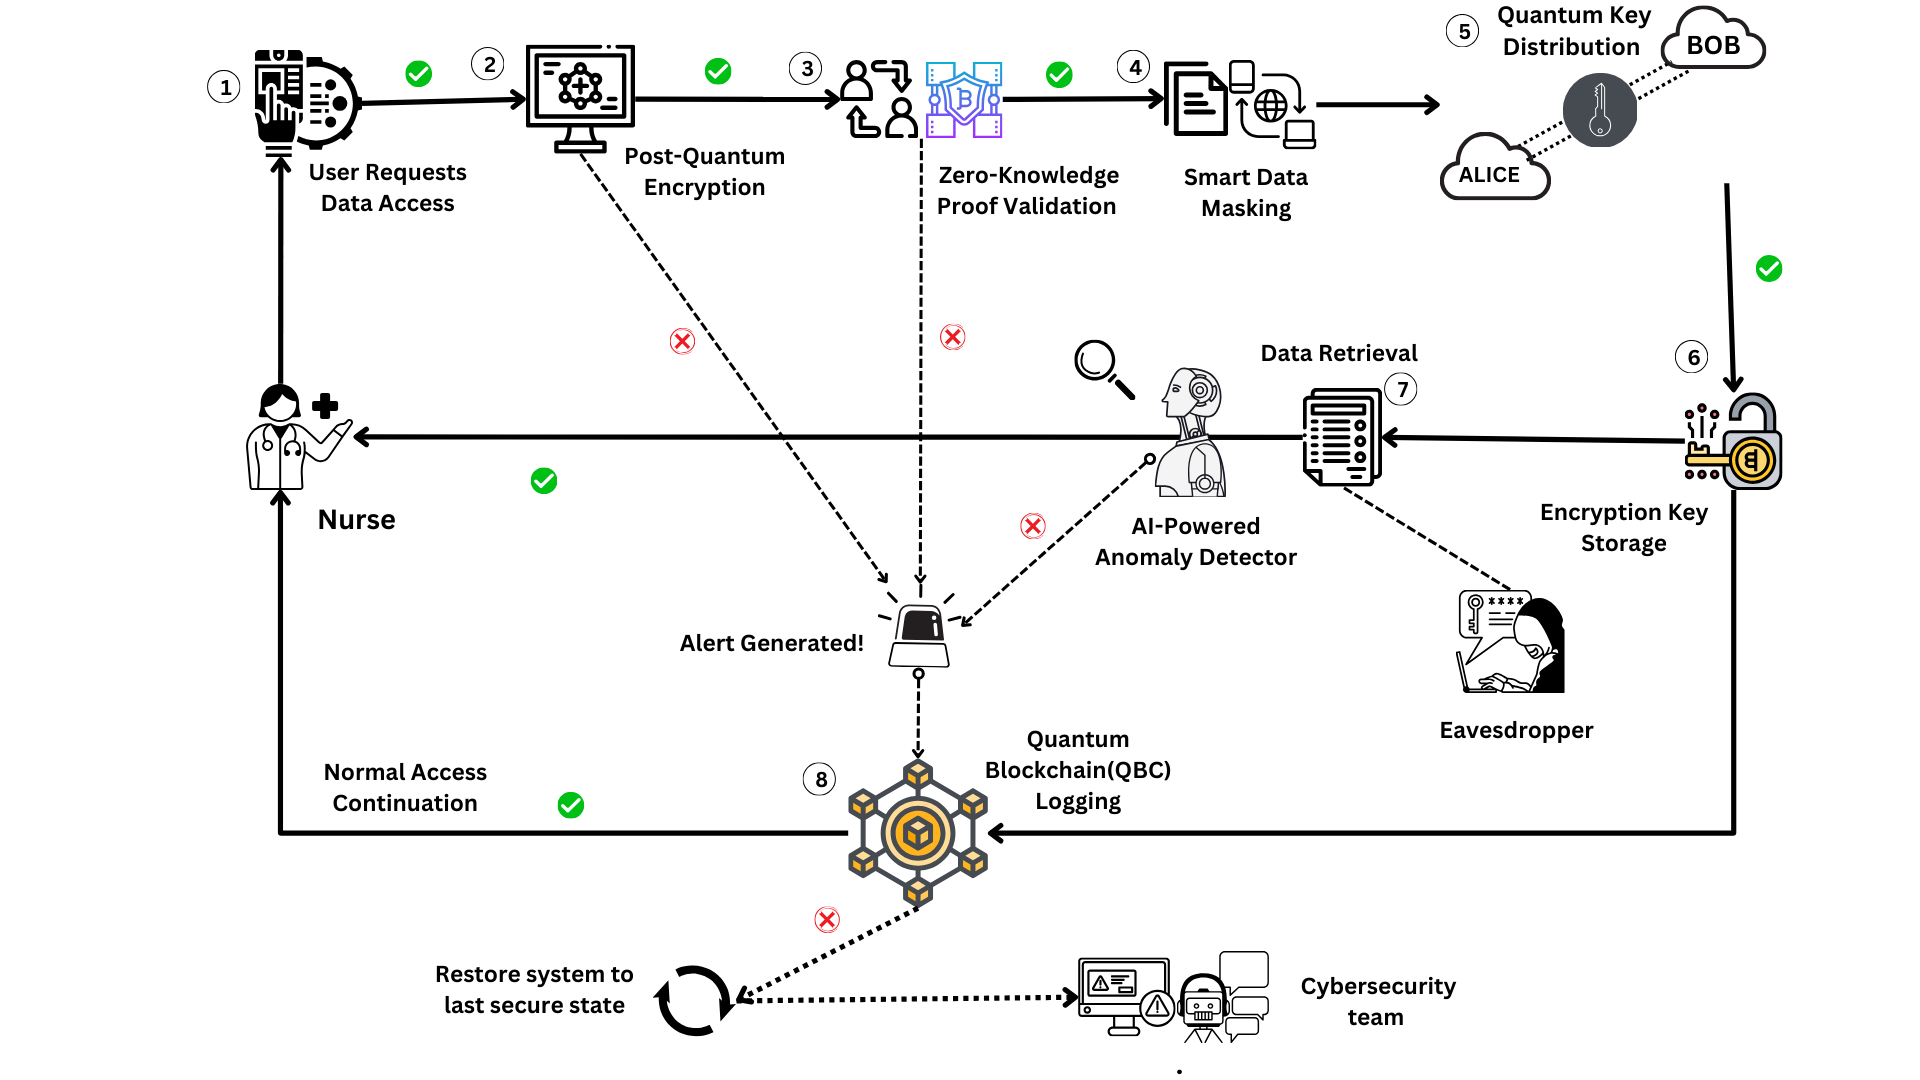
\includegraphics[width=13cm]{QKD.png}
\centering
\caption{Data Encryption, Anomaly Detection, and Quantum Key Distribution.}
  \label{fig:Data access}
\end{figure}



%%%%%%%%%%%%%%%%%%%%%%%%%%%%%%%%%%%%%%%%%%%%%%%%%%%%%




\subsection{Access Control for Patient Records}
To implement access control of access A blockchain-based role-based access control model is needed to ensure that only the users who are authorized can retrieve the record of patient\cite{bib17}. Suppose a user requests access to a patient's data.First their \texttt{user\_id} and \texttt{role} (e.g., doctor, nurse, administrator) are validated against the access permissions stored in the blockchain. Suppose \( P_k \) represents the patient record linked to a patient ID \( k \), stored in encrypted format on the blockchain. Consent validation is achieved after the patient’s \texttt{consent\_token}(denoted as \( C_k \)) is retrieved from the consent ledger. This system will verify the rightfulness of \( C_k \) using a digital signature and ensure \( \texttt{Verify}(C_k, S_k) = 1 \), where \( S_k \) is the patient’s signature key\cite{bib17}. Access is denied if \( C_k \) is invalid or expired. Moreover the system will determine whether the data type requested\( D_i \) is within the scope of the permissibility of user, defined as \( R(u_i) = \{D_1, D_2, \dots, D_n\} \), where \( u_i \) is the UserID and \( R \) is the permission set. If \( D_i \notin R(u_i) \), access is denied, and a blockchain transaction logs the event for transparency. 



%%%%%%%%%%%%%%%%%%%%%%%%%%%%%%%%%%%%%%%%%%%%%%%%%%%%%




\begin{algorithm}[h!]
\caption{Ultra-Secure User Authentication and Access Control [\ref{fig:User_Authentication}]}
\begin{algorithmic}[1]
\STATE 	\textbf{User Requests Access:} Login attempt detected, verification initiated.

\STATE 	\textbf{Quantum Biometric Authentication:} 
\IF{Biometric data matches} Proceed to Blockchain Verification.
\ELSE Trigger AI security alert, block user, log attempt on blockchain. \ENDIF

\STATE 	\textbf{Blockchain-Based Identity Verification:} 
\IF{User valid} Proceed to AI Behavioral Monitoring.
\ELSE Trigger AI security alert, block user, log attempt. \ENDIF

\STATE 	\textbf{AI-Based Behavioral Monitoring:} 
\IF{Behavior normal} Proceed to Access Control.
\ELSE Issue security challenge, restrict access. \ENDIF

\STATE 	\textbf{AI Security Challenge (If Suspicious Activity Detected):} 
\IF{User passes} Proceed to Access Control.
\ELSE Trigger alert, block user, log attempt. \ENDIF

\STATE 	\textbf{Role-Based Access Control \& Consent Validation:} 
\IF{Valid role \& consent} Grant access.
\ELSE Trigger alert, block user, log attempt. \ENDIF

\STATE 	\textbf{Secure Session Handling:} 
\IF{Session active} Maintain access.
\ELSE Trigger alert, block user, log attempt. \ENDIF

\STATE 	\textbf{Quantum Blockchain Logging:} 
\IF{No anomalies} Continue access.
\ELSE Revert system, notify cybersecurity team. \ENDIF
\end{algorithmic}
\end{algorithm}



For enhancement of efficiency, Merkle trees are implemented for verification of data. Record of each patient is hashed into a leaf node, and the root hash \( H_r \) ensures integrity of data. Access is granted only when all validations are successful, enabling the decryption of \( P_k \) using the authorized user’s private key \( K_u \), such that \( P_k = \texttt{Decrypt}(E(P_k), K_u) \). Failed attempts or anomalies are flagged for review and logged in the blockchain\cite{bib8}.




%%%%%%%%%%%%%%%%%%%%%%%%%%%%%%%%%%%%%%%%%%%%%%%%%%%%%





\subsection{Data Encryption and Privacy}
Classical cryptographic techniques are combined with quantum resistant algorithms to implement data encryption and privacy. This ensures a more advanced security. Let sensitive healthcare data generated from records of patient  or sensor inputs be indicated by \( H \). It must be encrypted before it is stored in the blockchain ledger. Firstly, an asymmetric encryption is implemented using an elliptic curve cryptography (ECC) framework. The plain text data \( H \) is encrypted by \( E_H = \texttt{Encrypt}(H, K_p) \), here \( K_p \) is the public key of recipient. Decryption is done through the corresponding private key \( K_s \) such that \( H = \texttt{Decrypt}(E_H, K_s) \). For ensuring post-quantum security lattice-based cryptography, particularly the NTRU (Number Theoretic Research Unit) algorithm is being used \cite{bib18}.Next, the ciphertext \( C_H \) is computed as \( C_H = \mathbf{M} \cdot \mathbf{F} + \mathbf{e} \mod q \),here \( \mathbf{M} \) is data matrix of patient, \( \mathbf{F} \) is secret key polynomial, \( \mathbf{e} \) is the error term, and \( q \) is a large prime modulus.

To store in blockchain the encrypted data \( E_H \) or \( C_H \) is integrated into the Merkle tree structure.It will increase the efficiency and integrity of data. Each transaction hash is a leaf node \( H_i = \texttt{Hash}(E_H) \), and the root hash \( H_r \) is determined iteratively as \( H_r = \texttt{Hash}(H_{2i} || H_{2i+1}) \). It is done to ensure resistance against tampering. For preserving auditability and transparency, metadata \( M_d \), like timestamps \( t \), access logs, and encryption keys, are integrated to the encrypted data. The blockchain validates \( M_d \) using a  proof protocol of zero knowledge\( ZKP(x) \), where \( x \) indicate the knowledge of the decryption key. This will ensure that encrypted data may be verified without revealing any information that is sensitive.

The privacy framework utilizes strategy of monitoring data access as shown in Figure \ref{fig:Data access}. Access request patterns \( A(t) \) are modeled as a time-series \( \{a_1, a_2, \dots, a_n\} \) and this help in anomaly detecting. AI Models like long short term memory networks(LSTM) analyze \( A(t) \)deviations from normal behavior. It warns as \( \texttt{Anomaly}(A(t)) = 1 \) if the deviation exceeds a predefined threshold \( \epsilon \). In the event of detecting such anomalies, an alert is produced. Then, the blockchain logs the incident for investigating further. This hybrid quantum-classical cryptographic and AI-supported measures are implemented to ensure privacy and integrity of data and also security against both classical and quantum threats.


%%%%%%%%%%%%%%%%%%%%%%%%%%%%%%%%%%%%%%%%%%%%%%%%%%%%%

\begin{algorithm}[h!]
\caption{Secure Data Encryption, Anomaly Detection, and Quantum Key Distribution}
\begin{algorithmic}[1]

\STATE \textbf{Step 1: User Requests Data Access}
\STATE User initiates a request to access encrypted medical data.
\STATE System verifies encryption status and logs unauthorized attempts.

\STATE \textbf{Step 2: Post-Quantum Encryption Processing}
\STATE System applies post-quantum encryption.
\IF{Encryption fails} 
    \STATE Trigger security alert, log failure, deny access. \textbf{Go to Step [7].}
\ENDIF

\STATE \textbf{Step 3: Zero-Knowledge Proof Validation}
\STATE Validate user credentials using zero-knowledge proof.
\IF{Validation fails} 
    \STATE Issue security challenge, log unauthorized request. \textbf{Go to Step [7].}
\ENDIF

\STATE \textbf{Step 4: Smart Data Masking for Role-Based Access}
\STATE Apply smart data masking based on user role.
\IF{Role unauthorized} 
    \STATE Block access, notify administrator, log violation. \textbf{Go to Step [7].}
\ENDIF

\STATE \textbf{Step 5: Quantum Key Distribution for Secure Encryption}
\STATE QKD refreshes encryption keys periodically.
\IF{Key compromise detected} 
    \STATE Regenerate encryption keys, log event.
\ENDIF

\STATE \textbf{Step 6: AI-Powered Anomaly Detection}
\STATE AI monitors access patterns, detects anomalies.
\IF{Anomaly detected} 
    \STATE Require additional authentication, restrict access, alert cybersecurity team.
\ENDIF


\STATE \textbf{Step 7: Quantum Blockchain Logging for Security and Audit}
\STATE Maintain immutable record of access and encryption activities.
\IF{Unauthorized modifications detected} 
    \STATE Deny access, revert to last secure state, alert cybersecurity team.
\ENDIF

\STATE \textbf{Final Security Enhancements}
\STATE System integrates post-quantum encryption, zero-knowledge proofs, AI anomaly detection, and blockchain logging to ensure security and mitigate threats.

\end{algorithmic}
\end{algorithm}

%%%%%%%%%%%%%%%%%%%%%%%%%%%%%%%%%%%%%%%%%%%%%%%%%%%%%





\subsection{AI-Based Anomaly Detection}
Anomaly can be detected using a framework that uses AI to identify unusual access patterns within the electronic healthcare records \cite{bib19}. Access request data \( A = \{a_1, a_2, \dots, a_n\} \)that consists of user IDs \( u \), timestamps \( t \), resource IDs \( r \) and device IDs \( d \) are continuously collected. From these data and records, feature vectors \( x_i \) are determined such as frequencyv of access, time intervals and behavior patterns of user. A machine learning model \( M \) is employed to classify the patterns into normal or abnormal behaviors based on past labeled data \( D = \{(x_i, y_i)\}_{i=1}^N \). Here \( y_i \) represents whether the behavior is normal (0) or anomalous (1). The AI model is trained by minimizing the loss function \( \mathcal{L}(M(D)) \)and by using classification algorithms like decision trees, random forests or neural networks\cite{bib18}.

After the model is trained it determines the probability of anomaly \( P(y=1|x_j) \) for every new access request \( x_j \). If the probability is greater a predefined threshold \( \theta \), the access request is rejected as abnormal and an alert is created. Moreover the anomaly is logged on the blockchain for transparency and audit purposes.As the time passes and as new data is available, the model is again trained to increase its accuracy.This will ensure the adaptive monitoring of the evolving access patterns. Clustering algorithms, for example k-means, are implemented for grouping similar anomalies and decrease false positives\cite{bib20}.

This approach will make sure the real time detection of unauthorized access or abnormal behavior. This will in turn enhance the security of the healthcare system by making  monitoring intelligent beside cryptographic defenses.



%%%%%%%%%%%%%%%%%%%%%%%%%%%%%%%%%%%%%%%%%%%%%%%%%%%%%

\subsection{Quantum Key Distribution for Secure Communication}
Quantum Key Distribution (QKD) is utilized for secure exchange of encryption keys between healthcare providers and patients\cite{bib21}. The QKD protocol such as BB84 or E91 allows the secure generation and exchange of symmetric keys over a quantum channel. Initially, a quantum state \( |\psi\rangle \) is prepared and transmitted through a quantum channel between the healthcare provider and patient. In the key generation procedure, information is encoded into quantum bits (qubits) and then it is transmitted using the property of polarization or quantum entanglement.

Upon receiving, the qubits are measured using a basis selected at random by both parties(say Alice and Bob). These observation are then compared over a classical channel inorder to produce a shared secret key \( K_{shared} \)\cite{bib21}. Any eavesdropping attempt disturbs the quantum state leading to its collapse.This is detectable because of the No-cloning theorem\cite{bib11}. When an eavesdropper is detected, the system dismisses that key exchange and the procedure is conducted once again. Thus the system ensures that the communication is secure.

The integrity of the quantum key \( K_{shared} \) is validated with the help of a checksum or hash function. Now, if validation fails, the system will return an error and will end the communication process. If it is successful, the key generated is used to encrypt and decrypt healthcare data using symmetric encryption techniques like AES-256\cite{bib22}. The quantum keys are regularly refreshed to ensure long-term security against quantum attacks and logs of key exchange events are stored on the blockchain for transparency and future auditability.

This method will make sure that the communication channel between healthcare providers and patients become secure even against quantum threats besides preserving the integrity of sensitive health data.




%%%%%%%%%%%%%%%%%%%%%%%%%%%%%%%%%%%%%%%%%%%%%%%%%%%%%

\begin{table}[h!]
    \centering
    \caption{Challenges and Proposed Solutions in AI-Based Quantum Healthcare Security}
    \label{tab:challenges_solutions}
    \begin{tabular}{|p{2cm}|p{4.8cm}|p{4.8cm}|}
        \hline
        \textbf{Topic} & \textbf{Challenge} & \textbf{Proposed Solution} \\
        \hline
        \textbf{Quantum Cryptography} & High computational cost of quantum-resistant cryptographic algorithms & Development of hardware-accelerated cryptographic processors and efficient key management strategies \\
        \hline
        \textbf{Blockchain Scalability} & Managing large-scale healthcare data on blockchain introduces latency and storage overhead & Implementation of sharding, off-chain storage techniques, and lightweight blockchain protocols \\
        \hline
        \textbf{Quantum Key Distribution (QKD)} & Secure and practical deployment of QKD in real-world healthcare environments & Use of hybrid QKD architectures with quantum-secure relay nodes and noise-resistant transmission techniques \\
        \hline
        \textbf{AI-Driven Security} & Lack of standardized frameworks for AI-driven anomaly detection in healthcare security & Development of benchmark datasets and federated learning models trained on privacy-preserving decentralized datasets \\
        \hline
        \textbf{Adversarial AI Attacks} & Risk of adversarial AI compromising authentication and access control systems & Adoption of adversarial training, GAN-based security enhancements, and robust AI defense mechanisms \\
        \hline
        \textbf{Regulatory Compliance} & Ensuring dynamic patient consent management while complying with HIPAA, GDPR & Integration of AI-driven smart contracts and zero-knowledge proof-based consent mechanisms \\
        \hline
        \textbf{Post-Quantum Security} & Vulnerability of existing encryption techniques to future quantum attacks & Adoption of lattice-based cryptography, NTRUEncrypt, and RLWE-based encryption for long-term quantum security \\
        \hline
    \end{tabular}
\end{table}

%%%%%%%%%%%%%%%%%%%%%%%%%%%%%%%%%%%%%%%%%%%%%%%%%%%%%

\subsection{Patient Data Access Logging and Audit}
Data access of patient is logged to ensure transparency and auditability\cite{bib22}. Each access request to healthcare data is recorded on the blockchain using the following details: the user \( user\_id \), the patient \( patient\_id \), the data accessed \( data\_accessed \), the timestamp \( t \), the device used \( device\_id \), and the consent status \( consent\_token \). Dexter's log is stored on the blockchain as a transaction. This ensures immutability of data and prevents tampering.

For maintenance of compliance with healthcare regulations such as HIPAA, the access logs are audited periodically. The audit process will be checking for any unauthorized access attempts by comparison of logged access events with predefined access rules and user roles. For an unauthorized access if detected, the system generated an alert and the security team is notified. Anomaly detection models can be integrated to detect abnormal access patterns or deviations from normal behavior,stimulating an investigation if necessary.


The blockchain will make sure that the logs are tamper proof and are easily auditable by external auditors. This provides an additional layer of security and trust. The audit trail can be accessed using cryptographic proofs. Thus without disclosing sensitive data, verification of the log entries can be conducted and this in turn helps in protecting patient privacy.

This comprehensive logging and auditing mechanism would ensure that all access to patient data is tracked and monitored. The main focus is to enhance security and regulatory compliance.




%%%%%%%%%%%%%%%%%%%%%%%%%%%%%%%%%%%%%%%%%%%%%%%%%%%%%

\subsection{Continuous Monitoring and Updates}
To maintain consistency in the security of the healthcare system, it is necessary to regularly monitor it. AI models are implemented to detect the possible threats such as new attack vectors or attempts of hacking\cite{bib23}. These models should be trained using a dynamic dataset that is periodically updated to improve the accuracy of detection. The system continuously analyzes access request data, system logs and behavioral patterns to detect potential security breaches in real-time. If an abnormality is detected an alert will be generated, and appropriate action will be taken to remove the threat.

Simultaneously the integrity of the blockchain ledger is continuously checked. A hash of the blockchain is periodically compared against the expected hash to detect unauthorized tampering. If any discrepancy is found the system responds by rejected any further access to compromised data and informing the security team\cite{bib16}.

Quantum encryption protocols are also updated periodically to remain resilient against advances in quantum computing. As quantum-safe algorithms evolve, they are integrated into the system to ensure the long-term security of encrypted healthcare data. Moreover, quantum keys are periodically refreshed to decrease the risk of key compromise.

These continuous monitoring and update mechanism will provide a robust defense against evolving threats and thus ensure that the system remains secure and also resilient over time.









%%%%%%%%%%%%%%%%%%%%%%%%%%%%%%%%%%%%%%%%%%%%%%%%%%%%%

\section{Conclusion}
This paper has explored the integration of advanced AI mechanism,Blockchain and Quantum cryptography to address the security challenges in healthcare systems. The proposed framework utilizes quantum key distribution (QKD), blockchain, and machine learning algorithms to generate a highly secure, tamper-proof, and privacy-protected environment to manage sensitive data of patient. Using the AI-driven anomaly detection and advanced encryption techniques that are Quantum based, we aim to make sure the integrity of data and also safeguard against the future quantum threats. Moreover, use of decentralized mechanisms for authentication and continuous monitoring enables dynamic protection for healthcare environments. Our contributions focuses on interconnecting the gap between classical and quantum security besides advancing the role of AI in healthcare. It also provides practical solutions to increase the scalability and efficiency for secure healthcare data management. The Quantum encryption protocols nees refinement in the future and optimization of blockchain scalability is also necessary. Finally, the expansion of AI driven threat detection models for real world healthcare applications is also to be considered.

%%%%%%%%%%%%%%%%%%%%%%%%%%%%%%%%%%%%%%%%%%%%%%%%%%%%%









 \bibliography{references}% common bib file
%% if required, the content of .bbl file can be included here once bbl is generated
%%\input sn-article.bbl


\end{document}
